\documentclass[11pt,a4paper]{article}

% ============================================
% PACKAGES
% ============================================
\usepackage[utf8]{inputenc}
\usepackage[T1]{fontenc}
\usepackage{lmodern}
\usepackage[margin=1in]{geometry}
\usepackage{graphicx}
\usepackage{xcolor}
\usepackage{titlesec}
\usepackage{hyperref}
\usepackage{fancyhdr}
\usepackage{amsmath, amssymb}
\usepackage{booktabs}
\usepackage{tabularx}
\usepackage{longtable}
\usepackage{enumitem}
\usepackage{tikz}
\usepackage{tcolorbox}
\usepackage{float}
\usepackage{listings}
\usepackage{caption}
\usepackage{setspace}
\usepackage{multicol}
\usepackage{fontawesome5}
\usepackage{etoolbox}

% ============================================
% COLOR DEFINITIONS
% ============================================
\definecolor{monadPurple}{RGB}{134, 65, 244}
\definecolor{monadDark}{RGB}{30, 20, 50}
\definecolor{wanderifyAccent}{RGB}{0, 255, 200}
\definecolor{wanderifyGold}{RGB}{255, 215, 0}
\definecolor{successGreen}{RGB}{34, 197, 94}
\definecolor{warningOrange}{RGB}{249, 115, 22}
\definecolor{dangerRed}{RGB}{239, 68, 68}
\definecolor{codeBackground}{RGB}{40, 44, 52}
\definecolor{linkBlue}{RGB}{59, 130, 246}

% ============================================
% HYPERREF SETUP
% ============================================
\hypersetup{
    colorlinks=true,
    linkcolor=monadPurple,
    filecolor=monadPurple,
    urlcolor=linkBlue,
    citecolor=monadPurple,
    pdftitle={Wanderify Protocol Whitepaper},
    pdfauthor={Wanderify Labs},
    pdfsubject={Travel-to-Earn Web3 dApp},
    pdfkeywords={Monad, Web3, Travel, Blockchain, DeFi, NFT}
}

% ============================================
% TIKZ LIBRARIES
% ============================================
\usetikzlibrary{shapes.geometric, arrows.meta, positioning, shadows, calc, decorations.pathreplacing}

% ============================================
% TCOLORBOX STYLES
% ============================================
\tcbuselibrary{skins, breakable}

\newtcolorbox{highlightbox}[1][]{
    enhanced,
    colback=monadPurple!5,
    colframe=monadPurple,
    arc=4pt,
    boxrule=1pt,
    left=10pt,
    right=10pt,
    top=10pt,
    bottom=10pt,
    #1
}

\newtcolorbox{warningbox}[1][]{
    enhanced,
    colback=warningOrange!5,
    colframe=warningOrange,
    arc=4pt,
    boxrule=1pt,
    left=10pt,
    right=10pt,
    top=10pt,
    bottom=10pt,
    #1
}

\newtcolorbox{successbox}[1][]{
    enhanced,
    colback=successGreen!5,
    colframe=successGreen,
    arc=4pt,
    boxrule=1pt,
    left=10pt,
    right=10pt,
    top=10pt,
    bottom=10pt,
    #1
}

\newtcolorbox{formulabox}[1][]{
    enhanced,
    colback=monadDark!5,
    colframe=monadDark,
    arc=4pt,
    boxrule=1.5pt,
    left=15pt,
    right=15pt,
    top=15pt,
    bottom=15pt,
    #1
}

% ============================================
% LISTINGS SETUP
% ============================================
\lstdefinestyle{soliditystyle}{
    backgroundcolor=\color{codeBackground},
    basicstyle=\ttfamily\footnotesize\color{white},
    keywordstyle=\color{monadPurple}\bfseries,
    stringstyle=\color{successGreen},
    commentstyle=\color{gray}\itshape,
    numbers=left,
    numberstyle=\tiny\color{gray},
    stepnumber=1,
    numbersep=8pt,
    frame=single,
    framesep=5pt,
    rulecolor=\color{monadPurple},
    breaklines=true,
    captionpos=b,
    showstringspaces=false,
    tabsize=2,
    keywords={contract, function, public, private, internal, external, view, pure, payable, returns, return, if, else, for, while, struct, mapping, event, emit, require, revert, modifier, constructor, address, uint256, bool, bytes32, string, memory, storage, calldata}
}
\lstset{style=soliditystyle}

% ============================================
% TITLE FORMATTING
% ============================================
\titleformat{\section}
    {\normalfont\LARGE\bfseries\color{monadPurple}}
    {\thesection.}
    {0.5em}
    {}
    [\titlerule]

\titleformat{\subsection}
    {\normalfont\Large\bfseries\color{monadDark}}
    {\thesubsection}
    {0.5em}
    {}

\titleformat{\subsubsection}
    {\normalfont\large\bfseries\color{monadPurple!80}}
    {\thesubsubsection}
    {0.5em}
    {}

% ============================================
% HEADER & FOOTER
% ============================================
\pagestyle{fancy}
\fancyhf{}
\fancyhead[L]{\textcolor{monadPurple}{\textbf{Wanderify Protocol}}}
\fancyhead[R]{\textcolor{gray}{Whitepaper v1.0}}
\fancyfoot[C]{\thepage}
\renewcommand{\headrulewidth}{0.5pt}
\renewcommand{\footrulewidth}{0.3pt}

% ============================================
% DOCUMENT BEGIN
% ============================================
\begin{document}

% ============================================
% TITLE PAGE
% ============================================
\begin{titlepage}
    \centering
    \vspace*{1cm}
    
    % Logo placeholder with TikZ
    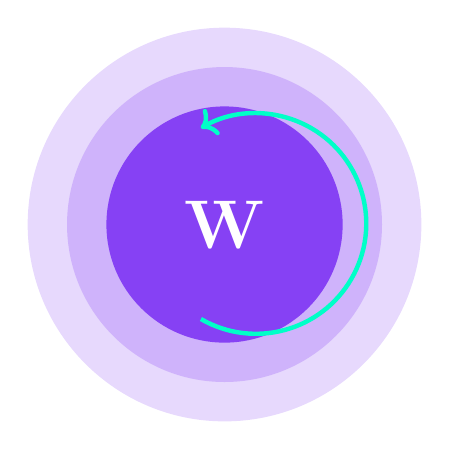
\begin{tikzpicture}
        \fill[monadPurple!20] (0,0) circle (2.5cm);
        \fill[monadPurple!40] (0,0) circle (2cm);
        \fill[monadPurple] (0,0) circle (1.5cm);
        \node[white, font=\Huge\bfseries] at (0,0) {W};
        \draw[wanderifyAccent, ultra thick, ->] (-0.3,-1.2) arc (-120:120:1.4);
    \end{tikzpicture}
    
    \vspace{1.5cm}
    
    {\Huge\bfseries\textcolor{monadPurple}{WANDERIFY}}\\[0.5cm]
    {\Large\textit{From On-Chain to On-Ground}}\\[0.3cm]
    {\large\textcolor{gray}{Travel-to-Earn Protocol Whitepaper}}
    
    \vspace{2cm}
    
    \begin{tcolorbox}[
        enhanced,
        colback=monadPurple!5,
        colframe=monadPurple,
        arc=8pt,
        boxrule=2pt,
        width=0.85\textwidth,
        halign=center
    ]
        \Large\bfseries
        \textcolor{monadDark}{Stake. Travel. Prove. Earn.}\\[0.5cm]
        \normalsize
        Transform your journeys into verifiable, rewarding on-chain adventures.
    \end{tcolorbox}
    
    \vspace{2cm}
    
    \begin{minipage}{0.7\textwidth}
        \centering
        \begin{tabular}{rl}
            \textbf{Version:} & 1.0 \\
            \textbf{Network:} & Monad Blockchain \\
            \textbf{Date:} & January 2026 \\
            \textbf{Contract:} & \texttt{0x26c5...1eeD0}\\
        \end{tabular}
    \end{minipage}
    
    \vfill
    
    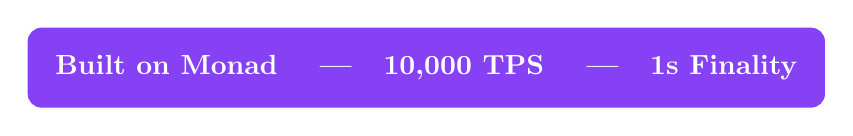
\begin{tikzpicture}
        \node[rounded corners=5pt, fill=monadPurple, text=white, inner sep=10pt, font=\bfseries] 
            {Built on Monad \quad|\quad 10,000 TPS \quad|\quad 1s Finality};
    \end{tikzpicture}
    
\end{titlepage}

% ============================================
% TABLE OF CONTENTS
% ============================================
\tableofcontents
\newpage

% ============================================
% SECTION 1: EXECUTIVE SUMMARY
% ============================================
\section{Executive Summary}

\begin{highlightbox}
\textbf{The Pitch:} Wanderify is the world's first \textbf{travel-to-earn Web3 dApp} that transforms journeys into verifiable, rewarding on-chain adventures. Your travel is not just a memory—it's a \textbf{transaction}.
\end{highlightbox}

\vspace{0.5cm}

Wanderify introduces a revolutionary paradigm where:
\begin{itemize}[leftmargin=2cm]
    \item[\faMapMarkerAlt] You \textbf{stake before you go}, proving genuine travel intent
    \item[\faGlobeAmericas] You \textbf{prove arrival with GPS validation}, connecting digital commitment to physical presence
    \item[\faTrophy] You \textbf{earn rewards from circular pools} that grow stronger with community participation
    \item[\faMedal] You \textbf{receive Journey NFTs} as permanent, tradeable proof of your accomplishments
\end{itemize}

\vspace{0.5cm}

\begin{center}
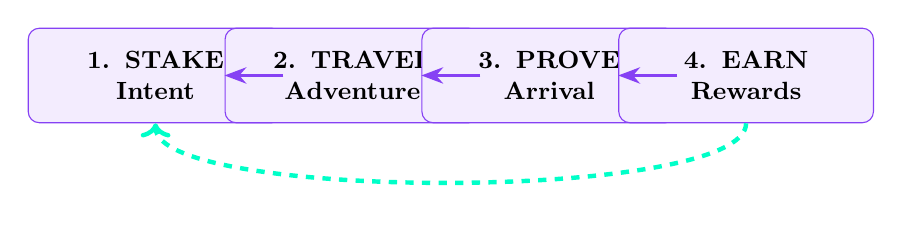
\begin{tikzpicture}[
    node distance=2.5cm,
    box/.style={rectangle, rounded corners, draw=monadPurple, fill=monadPurple!10, text width=3cm, minimum height=1.2cm, align=center, font=\small\bfseries},
    arrow/.style={-{Stealth[scale=1.2]}, thick, monadPurple}
]
    \node[box] (stake) {1. STAKE\\Intent};
    \node[box, right of=stake] (travel) {2. TRAVEL\\Adventure};
    \node[box, right of=travel] (prove) {3. PROVE\\Arrival};
    \node[box, right of=prove] (earn) {4. EARN\\Rewards};
    
    \draw[arrow] (stake) -- (travel);
    \draw[arrow] (travel) -- (prove);
    \draw[arrow] (prove) -- (earn);
    
    \draw[wanderifyAccent, ultra thick, dashed, ->] (earn.south) .. controls +(0,-1) and +(0,-1) .. (stake.south);
\end{tikzpicture}
\end{center}

\subsection{Key Metrics}

\begin{center}
\begin{tabular}{|c|c|c|c|}
    \hline
    \rowcolor{monadPurple!20}
    \textbf{Parameter} & \textbf{Value} & \textbf{Parameter} & \textbf{Value} \\
    \hline
    Base Reward & 0.002 TMON & Platform Fee & 4\% \\
    \hline
    Min Stake Duration & 15 days & Claim Window & 24 hours \\
    \hline
    Pool Cap per Win & 10\% max & Check-in Radius & 50 meters \\
    \hline
\end{tabular}
\end{center}

% ============================================
% SECTION 2: THE PROBLEM
% ============================================
\section{The Problem}

The travel industry generates over \$9 trillion annually, yet the intersection of travel and blockchain remains largely untapped. Current challenges prevent the creation of a sustainable travel-to-earn ecosystem:

\subsection{Unverifiable Travel Experiences}

\begin{warningbox}
\textbf{Travel today = photos and posts, but nothing verifiable or valuable on-chain.}
\end{warningbox}

Social media posts can be faked. GPS data can be spoofed. There exists no trustworthy protocol for proving that a person was physically present at a specific location at a specific time.

\subsection{Weak Sustainability Models}

Existing "travel-to-earn" applications suffer from:
\begin{itemize}
    \item \textbf{Inflationary token models} — Rewards are minted infinitely, leading to value degradation
    \item \textbf{No commitment mechanism} — Users can claim rewards without genuine travel intent
    \item \textbf{Centralized verification} — Single points of failure in proof systems
\end{itemize}

\subsection{The Missing Link}

\begin{center}
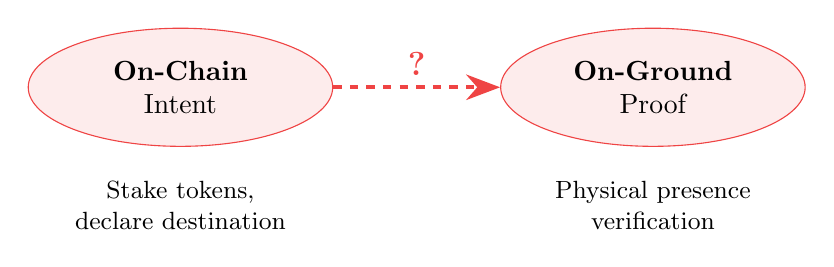
\begin{tikzpicture}[
    node distance=3cm,
    cloud/.style={ellipse, draw=dangerRed, fill=dangerRed!10, text width=2.5cm, align=center, minimum height=1.5cm},
    arrow/.style={-{Stealth[scale=1.2]}, ultra thick, dangerRed, dashed}
]
    \node[cloud] (onchain) {\textbf{On-Chain}\\Intent};
    \node[cloud, right of=onchain, xshift=3cm] (onground) {\textbf{On-Ground}\\Proof};
    
    \draw[arrow] (onchain) -- node[above, font=\large\bfseries, color=dangerRed] {?} (onground);
    
    \node[below of=onchain, node distance=1.5cm, font=\small, text width=3cm, align=center] {Stake tokens,\\declare destination};
    \node[below of=onground, node distance=1.5cm, font=\small, text width=3cm, align=center] {Physical presence\\verification};
\end{tikzpicture}
\end{center}

\textbf{No protocol exists that connects on-chain intent with on-ground proof of arrival.} This gap prevents the creation of trustless, self-sustaining travel reward systems.

% ============================================
% SECTION 3: THE SOLUTION
% ============================================
\section{The Wanderify Solution}

Wanderify solves the travel verification problem through an innovative combination of \textbf{stake-first economics} and \textbf{gamified proof-of-travel}.

\subsection{Core Mechanics}

\subsubsection{Place Value System (0–100)}

Each destination is assigned a \textbf{Place Value} score representing difficulty and desirability:

\begin{center}
\begin{tabular}{|c|l|c|c|}
    \hline
    \rowcolor{monadPurple!20}
    \textbf{ID} & \textbf{Destination} & \textbf{Place Value} & \textbf{Difficulty} \\
    \hline
    1 & Everest Base Camp, Nepal & 80 & \textcolor{dangerRed}{\textbf{Legendary}} \\
    \hline
    2 & Chadar Trek, Zanskar & 70 & \textcolor{warningOrange}{\textbf{Epic}} \\
    \hline
    3 & Hemkund Sahib \& Valley of Flowers & 60 & \textcolor{warningOrange}{\textbf{Hard}} \\
    \hline
    4 & Key Monastery, Spiti & 50 & \textcolor{warningOrange}{\textbf{Hard}} \\
    \hline
    5 & Havelock Island Circuit & 40 & \textcolor{wanderifyGold}{\textbf{Medium}} \\
    \hline
    6 & Jaisalmer Fort \& Sam Dunes & 30 & \textcolor{wanderifyGold}{\textbf{Medium}} \\
    \hline
    7 & IIIT Dharwad Campus & 20 & \textcolor{successGreen}{\textbf{Easy}} \\
    \hline
    8 & LNMIIT Jaipur Campus & 20 & \textcolor{successGreen}{\textbf{Easy}} \\
    \hline
\end{tabular}
\end{center}

\textbf{Higher Place Value = Higher Potential Rewards}

\subsubsection{15-Day Stake Commitment}

Users must lock their stake \textbf{at least 15 days before} the scheduled travel date. This mechanism ensures:
\begin{itemize}
    \item \textbf{Genuine Intent} — Spontaneous, unfounded claims are impossible
    \item \textbf{Economic Security} — Stakes cannot be withdrawn arbitrarily
    \item \textbf{Pool Stability} — Destination pools have predictable liquidity
\end{itemize}

\begin{highlightbox}
\textbf{Key Insight:} The more days between staking and travel, the more committed the traveler. Future versions may implement extended commitment bonuses.
\end{highlightbox}

\subsubsection{24-Hour Claim Window}

Upon reaching the travel date, users have exactly \textbf{24 hours} to:
\begin{enumerate}
    \item Navigate to within 50 meters of the destination
    \item Request GPS verification from the backend
    \item Submit the signed proof to the smart contract
    \item Receive their stake return + reward emission + Journey NFT
\end{enumerate}

\subsection{Circular Pool Economy}

Wanderify implements a self-sustaining, \textbf{circular pool system} that prevents reward drainage:

\begin{center}
\begin{tikzpicture}[
    node distance=2cm,
    pool/.style={rectangle, rounded corners, draw=monadPurple, fill=monadPurple!20, text width=3.5cm, minimum height=2cm, align=center},
    flow/.style={rectangle, rounded corners, draw=gray, fill=gray!10, text width=2.5cm, minimum height=1cm, align=center, font=\small},
    arrow/.style={-{Stealth[scale=1.2]}, thick}
]
    % Main flow
    \node[flow, fill=successGreen!20, draw=successGreen] (user) {\textbf{User Stake}\\1.0 TMON};
    \node[pool, right of=user, xshift=2.5cm] (pool) {\textbf{Destination Pool}\\96\% of stake\\grows over time};
    \node[flow, fill=monadPurple!20, draw=monadPurple, below of=user, yshift=-0.5cm] (treasury) {\textbf{Treasury}\\4\% fee};
    
    % Outcomes
    \node[flow, fill=successGreen!20, draw=successGreen, right of=pool, xshift=3cm, yshift=1cm] (success) {\faCheckCircle\ \textbf{SUCCESS}\\Stake + Reward\\+ Journey NFT};
    \node[flow, fill=dangerRed!20, draw=dangerRed, right of=pool, xshift=3cm, yshift=-1cm] (failure) {\faTimesCircle\ \textbf{FAILURE}\\Stake remains\\in pool};
    
    % Arrows
    \draw[arrow, successGreen] (user) -- node[above, font=\footnotesize] {96\%} (pool);
    \draw[arrow, monadPurple] (user) -- node[left, font=\footnotesize] {4\%} (treasury);
    \draw[arrow, successGreen] (pool) -- (success);
    \draw[arrow, dangerRed, dashed] (pool) -- (failure);
    \draw[arrow, dangerRed, ultra thick] (failure.south) .. controls +(0,-1) and +(0,-1) .. node[below, font=\footnotesize] {Fuels future winners} (pool.south);
\end{tikzpicture}
\end{center}

\begin{formulabox}
\textbf{Pool Mechanics:}
\begin{itemize}
    \item \textbf{96\%} of each stake → Destination-specific reward pool
    \item \textbf{4\%} of each stake → Protocol treasury (max 5\%)
    \item \textbf{Failures} leave their stake in the pool, growing rewards for future winners
    \item \textbf{Winners} receive their stake back + capped pool emission
\end{itemize}
\end{formulabox}

\subsection{Animated Navigation Experience}

As users approach their destination, Wanderify provides an immersive, \textbf{RPG-style navigation experience}:

\begin{center}
\begin{tikzpicture}[
    zone/.style={circle, draw, thick, minimum size=#1},
    zonelabel/.style={font=\small\bfseries}
]
    % Destination center
    \fill[wanderifyAccent!30] (0,0) circle (3cm);
    \fill[wanderifyAccent!50] (0,0) circle (2cm);
    \fill[wanderifyAccent!70] (0,0) circle (1cm);
    \fill[wanderifyAccent] (0,0) circle (0.4cm);
    
    % Zone labels
    \node[zonelabel, color=dangerRed] at (2.5, 2.5) {FAR ($>$500m)};
    \node[zonelabel, color=linkBlue] at (1.5, 1.5) {NEAR ($\leq$500m)};
    \node[zonelabel, color=warningOrange] at (0.6, 0.8) {CLOSE};
    \node[zonelabel, color=successGreen] at (0, -0.7) {READY};
    \node[font=\footnotesize] at (0, -1.1) {($\leq$50m)};
    
    % User avatar
    \fill[monadPurple] (2.2, -1.8) circle (0.2cm);
    \draw[monadPurple, ultra thick, dashed, ->] (2.2, -1.8) -- (0.3, -0.2);
    \node[font=\footnotesize, below] at (2.2, -2.1) {User};
    
    % Destination marker
    \node[font=\Large] at (0, 0) {\faMapMarkerAlt};
\end{tikzpicture}
\end{center}

\textbf{Navigation Features:}
\begin{itemize}
    \item Real-time distance updates using Haversine formula
    \item Color-coded proximity zones (FAR → NEAR → CLOSE → READY)
    \item Pulsing reward radius when check-in becomes available
    \item Avatar movement animation showing path to destination
\end{itemize}

% ============================================
% SECTION 4: TECHNICAL ARCHITECTURE
% ============================================
\section{Technical Architecture}

\subsection{System Overview}

\begin{center}
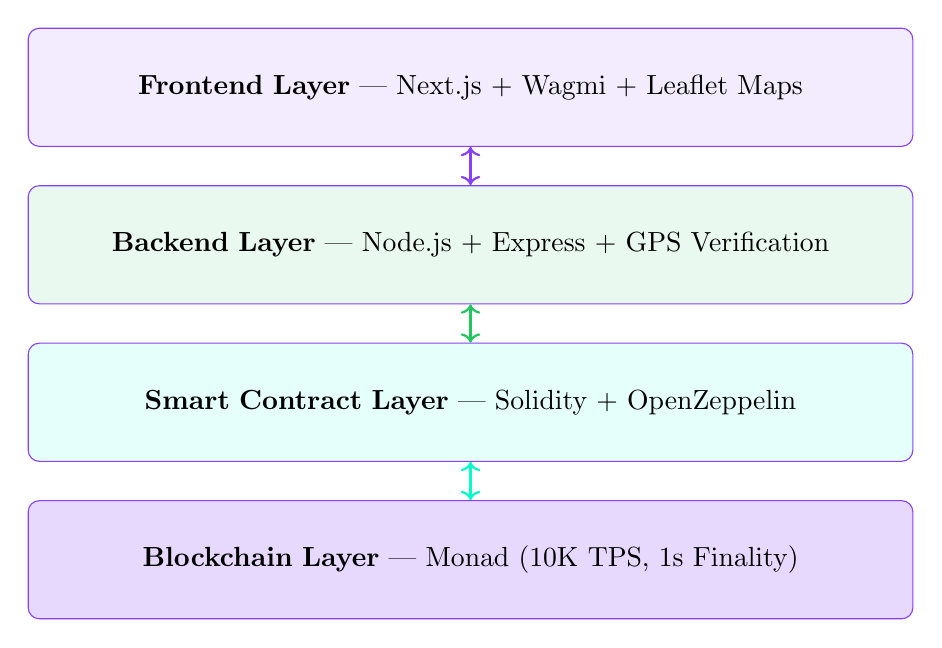
\begin{tikzpicture}[
    node distance=1.5cm,
    layer/.style={rectangle, rounded corners, draw=monadPurple, fill=#1, text width=11cm, minimum height=1.5cm, align=center},
    component/.style={rectangle, rounded corners, draw=gray, fill=white, text width=2.5cm, minimum height=0.8cm, align=center, font=\small}
]
    % Layers
    \node[layer=monadPurple!10] (frontend) {\textbf{Frontend Layer} — Next.js + Wagmi + Leaflet Maps};
    \node[layer=successGreen!10, below of=frontend, yshift=-0.5cm] (backend) {\textbf{Backend Layer} — Node.js + Express + GPS Verification};
    \node[layer=wanderifyAccent!10, below of=backend, yshift=-0.5cm] (contract) {\textbf{Smart Contract Layer} — Solidity + OpenZeppelin};
    \node[layer=monadPurple!20, below of=contract, yshift=-0.5cm] (blockchain) {\textbf{Blockchain Layer} — Monad (10K TPS, 1s Finality)};
    
    % Connections
    \draw[thick, monadPurple, <->] (frontend) -- (backend);
    \draw[thick, successGreen, <->] (backend) -- (contract);
    \draw[thick, wanderifyAccent, <->] (contract) -- (blockchain);
\end{tikzpicture}
\end{center}

\subsection{Smart Contract: WandryFi.sol}

The core protocol is implemented as a single, gas-optimized Solidity contract:

\begin{lstlisting}[caption=Core Contract Structure]
contract WandryFi is 
    ERC721, 
    ERC721URIStorage, 
    Ownable, 
    ReentrancyGuard, 
    Pausable 
{
    // Constants
    uint256 public constant MIN_STAKE_DURATION = 15 days;
    uint256 public constant BASE_REWARD = 2000000000000000; // 0.002 TMON
    uint256 public constant BETA = 50; // 0.5 scaled by 100
    uint256 public constant CLAIM_WINDOW = 1 days;
    
    // Core Data Structures
    struct Commitment {
        address user;
        uint256 amountInPool;
        uint256 travelDate;
        uint256 destinationId;
        bool isProcessed;
    }
    
    struct JourneyNFT {
        uint256 destinationId;
        uint256 completionDate;
        uint256 stakedAmount;
        uint256 rewardEarned;
        string destinationName;
    }
}
\end{lstlisting}

\subsubsection{Core Functions}

\begin{center}
\begin{tabular}{|p{3.5cm}|p{8cm}|}
    \hline
    \rowcolor{monadPurple!20}
    \textbf{Function} & \textbf{Description} \\
    \hline
    \texttt{stake(destId, date)} & Lock TMON with a destination and travel date commitment \\
    \hline
    \texttt{checkIn(signature)} & Submit verifier signature to claim rewards \\
    \hline
    \texttt{processFailure()} & Self-liquidate expired commitment (stake stays in pool) \\
    \hline
    \texttt{getUserCommitment()} & View active commitment details \\
    \hline
    \texttt{getPoolBalance(destId)} & Check destination pool balance \\
    \hline
    \texttt{getLeaderboard()} & Retrieve all users ranked by profit \\
    \hline
\end{tabular}
\end{center}

\subsection{Verification Pipeline}

The backend verification system implements multi-layer fraud prevention:

\begin{center}
\begin{tikzpicture}[
    node distance=1.2cm,
    step/.style={rectangle, rounded corners, draw=monadPurple, fill=monadPurple!10, text width=6cm, minimum height=1cm, align=center},
    check/.style={rectangle, rounded corners, draw=successGreen, fill=successGreen!10, text width=2.5cm, minimum height=0.6cm, align=center, font=\small},
    arrow/.style={-{Stealth[scale=1]}, thick, monadPurple}
]
    \node[step] (api) {\textbf{Step 1:} API Key Validation};
    \node[check, right of=api, xshift=3.5cm] (c1) {\faCheck\ Valid Key};
    
    \node[step, below of=api] (ip) {\textbf{Step 2:} IP Geolocation Match};
    \node[check, right of=ip, xshift=3.5cm] (c2) {\faCheck\ Country Match};
    
    \node[step, below of=ip] (vpn) {\textbf{Step 3:} VPN/Proxy Detection};
    \node[check, right of=vpn, xshift=3.5cm] (c3) {\faCheck\ No VPN};
    
    \node[step, below of=vpn] (gps) {\textbf{Step 4:} GPS Distance Check};
    \node[check, right of=gps, xshift=3.5cm] (c4) {\faCheck\ $\leq$ 50m};
    
    \node[step, below of=gps, fill=successGreen!20] (sign) {\textbf{Step 5:} Generate ECDSA Signature};
    
    \draw[arrow] (api) -- (ip);
    \draw[arrow] (ip) -- (vpn);
    \draw[arrow] (vpn) -- (gps);
    \draw[arrow] (gps) -- (sign);
    
    \draw[successGreen, thick] (api) -- (c1);
    \draw[successGreen, thick] (ip) -- (c2);
    \draw[successGreen, thick] (vpn) -- (c3);
    \draw[successGreen, thick] (gps) -- (c4);
\end{tikzpicture}
\end{center}

\subsubsection{Haversine Distance Formula}

GPS verification uses the \textbf{Haversine formula} for accurate spherical distance calculation:

\begin{formulabox}
\begin{equation*}
d = 2r \cdot \arcsin\left(\sqrt{\sin^2\left(\frac{\phi_2 - \phi_1}{2}\right) + \cos(\phi_1) \cdot \cos(\phi_2) \cdot \sin^2\left(\frac{\lambda_2 - \lambda_1}{2}\right)}\right)
\end{equation*}

Where:
\begin{itemize}
    \item $r$ = Earth's radius (6,371 km)
    \item $\phi_1, \phi_2$ = Latitudes of user and destination
    \item $\lambda_1, \lambda_2$ = Longitudes of user and destination
    \item $d$ = Distance between points
\end{itemize}

\textbf{Check-in Requirement:} $d \leq 50$ meters
\end{formulabox}

% ============================================
% SECTION 5: USER JOURNEY
% ============================================
\section{User Journey}

\subsection{Phase 1: Discover Destinations}

Users browse an interactive map displaying:
\begin{itemize}
    \item \textbf{Place Values} — Difficulty multipliers for each location
    \item \textbf{Pool Sizes} — Current reward pool balances
    \item \textbf{Success/Failure Stats} — Historical completion rates
    \item \textbf{Coordinates \& Descriptions} — Detailed destination information
\end{itemize}

\subsection{Phase 2: Stake Intent}

\begin{center}
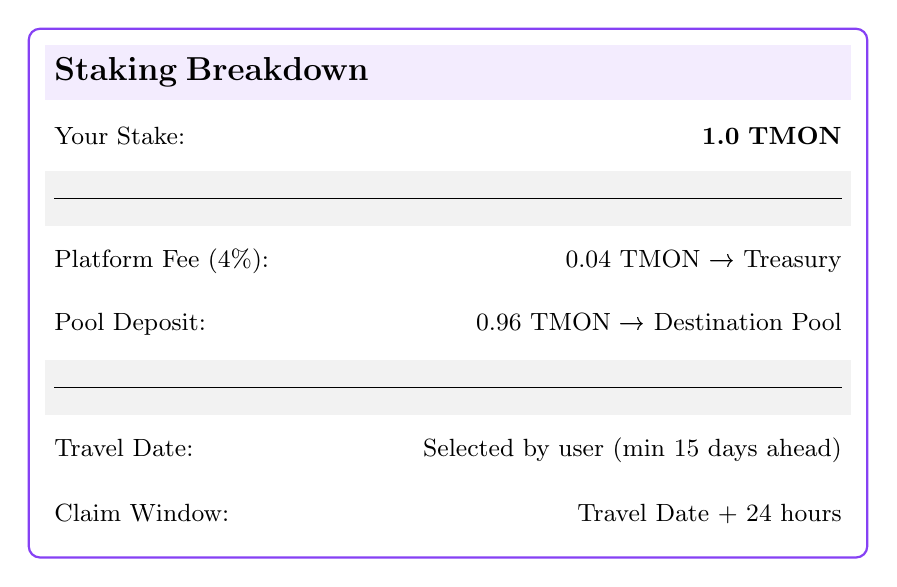
\begin{tikzpicture}[
    node distance=0.8cm,
    row/.style={rectangle, text width=10cm, minimum height=0.7cm, align=left, font=\small}
]
    \node[row, fill=monadPurple!10] (title) {\textbf{\large Staking Breakdown}};
    \node[row, below of=title] (stake) {Your Stake: \hfill \textbf{1.0 TMON}};
    \node[row, below of=stake, fill=gray!10] (sep) {\rule{\textwidth}{0.4pt}};
    \node[row, below of=sep] (fee) {Platform Fee (4\%): \hfill 0.04 TMON → Treasury};
    \node[row, below of=fee] (pool) {Pool Deposit: \hfill 0.96 TMON → Destination Pool};
    \node[row, below of=pool, fill=gray!10] (sep2) {\rule{\textwidth}{0.4pt}};
    \node[row, below of=sep2] (date) {Travel Date: \hfill Selected by user (min 15 days ahead)};
    \node[row, below of=date] (window) {Claim Window: \hfill Travel Date + 24 hours};
    
    \draw[monadPurple, thick, rounded corners] 
        ($(title.north west)+(-0.2,0.2)$) rectangle ($(window.south east)+(0.2,-0.2)$);
\end{tikzpicture}
\end{center}

\subsection{Phase 3: Travel \& Navigate}

The animated navigation system guides users to their destination:

\begin{enumerate}
    \item \textbf{Map Centers} — Auto-adjusts view to show both user and destination
    \item \textbf{User Avatar} — Animated marker with pulsing effect
    \item \textbf{Path Visualization} — Cyan polyline connecting user to target
    \item \textbf{Distance Display} — Real-time distance in meters/kilometers
    \item \textbf{Progress Bar} — Visual progress toward the reward zone
\end{enumerate}

\subsection{Phase 4: Check-In \& Verify}

\begin{center}
\begin{tikzpicture}[
    node distance=1.5cm,
    entity/.style={rectangle, rounded corners, draw=monadPurple, fill=monadPurple!10, text width=2.5cm, minimum height=1.5cm, align=center},
    arrow/.style={-{Stealth[scale=1]}, thick}
]
    \node[entity] (user) {\faUser\\\textbf{User}\\Location};
    \node[entity, right of=user, xshift=3cm] (backend) {\faServer\\\textbf{Backend}\\Verifier};
    \node[entity, right of=backend, xshift=3cm] (contract) {\faFileContract\\\textbf{Smart}\\Contract};
    
    \draw[arrow, monadPurple] (user) -- node[above, font=\footnotesize] {GPS coords} (backend);
    \draw[arrow, successGreen] (backend) -- node[above, font=\footnotesize] {Signature} (user);
    \draw[arrow, monadPurple] (user.south) .. controls +(0,-1) and +(0,-1) .. 
        node[below, font=\footnotesize] {checkIn(signature)} (contract.south);
    \draw[arrow, wanderifyAccent] (contract.north) .. controls +(0,1) and +(0,1) .. 
        node[above, font=\footnotesize] {Payout + NFT} (user.north);
\end{tikzpicture}
\end{center}

\subsection{Phase 5: Rewards}

Upon successful verification, users receive:

\begin{successbox}
\begin{enumerate}
    \item \textbf{Stake Return:} Full pool deposit returned (96\% of original stake)
    \item \textbf{Pool Emission:} Reward calculated based on Place Value
    \item \textbf{Journey NFT:} ERC-721 token commemorating the adventure
    \item \textbf{Leaderboard Points:} Profit added to user's ranking score
\end{enumerate}
\end{successbox}

% ============================================
% SECTION 6: TOKENOMICS
% ============================================
\section{Reward System \& Tokenomics}

\subsection{Emission Formula}

Wanderify uses a sustainable, capped reward emission system:

\begin{formulabox}
\begin{equation*}
E = \min\left(\text{BaseReward} \times \left(1 + \frac{\beta \times \text{PlaceValue}}{100}\right), \text{Pool} \times 10\%\right)
\end{equation*}

\begin{equation*}
\text{Total Payout} = \text{AmountInPool} + E
\end{equation*}

\textbf{Constants:}
\begin{itemize}
    \item $\text{BaseReward} = 0.002$ TMON
    \item $\beta = 50$ (representing 0.5 multiplier)
    \item $\text{Pool Cap} = 10\%$ of destination pool
\end{itemize}
\end{formulabox}

\subsection{Example Calculation}

\begin{center}
\begin{tabular}{|l|r|}
    \hline
    \rowcolor{monadPurple!20}
    \textbf{Parameter} & \textbf{Value} \\
    \hline
    User Stake & 1.0 TMON \\
    \hline
    Platform Fee (4\%) & 0.04 TMON \\
    \hline
    AmountInPool & 0.96 TMON \\
    \hline
    Destination & Everest Base Camp \\
    \hline
    Place Value & 80 \\
    \hline
    Pool Balance & 5.0 TMON \\
    \hline
\end{tabular}
\end{center}

\textbf{Calculation:}
\begin{align*}
\text{PlaceValueBonus} &= 0.002 \times \frac{100 + 50 \times 80}{100} \\
&= 0.002 \times \frac{100 + 4000}{100} \\
&= 0.002 \times 41 = 0.082 \text{ TMON}
\end{align*}

\begin{align*}
\text{PoolCap} &= 5.0 \times 10\% = 0.5 \text{ TMON} \\
\text{Emission } (E) &= \min(0.082, 0.5) = 0.082 \text{ TMON} \\
\text{Total Payout} &= 0.96 + 0.082 = \textbf{1.042 TMON}
\end{align*}

\begin{successbox}
\textbf{Result:} User earns \textbf{0.042 TMON profit} (4.2\% gain) on a 1.0 TMON stake to Everest Base Camp!
\end{successbox}

\subsection{Sustainability Mechanics}

\begin{center}
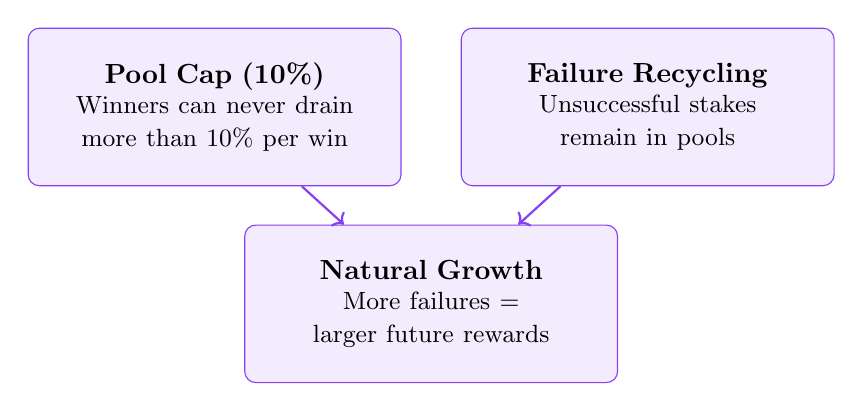
\begin{tikzpicture}[
    node distance=2cm,
    mech/.style={rectangle, rounded corners, draw=monadPurple, fill=monadPurple!10, text width=4.5cm, minimum height=2cm, align=center}
]
    \node[mech] (cap) {\textbf{Pool Cap (10\%)}\\\small Winners can never drain\\more than 10\% per win};
    \node[mech, right of=cap, xshift=3.5cm] (failures) {\textbf{Failure Recycling}\\\small Unsuccessful stakes\\remain in pools};
    \node[mech, below of=cap, yshift=-0.5cm, xshift=2.75cm] (growth) {\textbf{Natural Growth}\\\small More failures =\\larger future rewards};
    
    \draw[monadPurple, thick, ->] (cap) -- (growth);
    \draw[monadPurple, thick, ->] (failures) -- (growth);
\end{tikzpicture}
\end{center}

% ============================================
% SECTION 7: WHY MONAD
% ============================================
\section{Why Monad + Wanderify}

\begin{highlightbox}
\textbf{Monad is the ideal blockchain for Wanderify.} The protocol requires frequent microtransactions—staking, check-ins, NFT minting, and reward distribution. Monad's architecture makes these operations fast, cheap, and scalable.
\end{highlightbox}

\subsection{Monad Advantages}

\begin{center}
\begin{tabular}{|l|l|l|}
    \hline
    \rowcolor{monadPurple!20}
    \textbf{Monad Strength} & \textbf{Specification} & \textbf{Wanderify Benefit} \\
    \hline
    Throughput & 10,000 TPS & Handle global user base simultaneously \\
    \hline
    Finality & 1 second & Instant stake confirmation \& check-ins \\
    \hline
    Gas Fees & Ultra-low & Affordable microtransactions for all users \\
    \hline
    Compatibility & Full EVM & Standard Solidity development \& tooling \\
    \hline
    Architecture & Parallel Execution & No congestion during peak usage \\
    \hline
\end{tabular}
\end{center}

\subsection{Consumer Showcase}

\begin{center}

\begin{tikzpicture}
    \node[
        rectangle, 
        rounded corners=10pt, 
        draw=monadPurple, 
        fill=monadPurple!10, 
        text width=12cm, 
        minimum height=2cm, 
        align=center,
        font=\Large\itshape
    ] {
        ``Every step becomes a transaction.\\Every arrival becomes a reward.''
    };
\end{tikzpicture}
\end{center}

% ============================================
% SECTION 8: UNIQUE VALUE PROPOSITION
% ============================================
\section{What Makes Wanderify Unique}

\subsection{On-Chain to On-Ground Bridge}

\begin{center}
\begin{tabular}{|l|p{8cm}|}
    \hline
    \rowcolor{monadPurple!20}
    \textbf{Feature} & \textbf{Implementation} \\
    \hline
    GPS Validation & Haversine formula calculates distance; 50m radius required \\
    \hline
    IP Geolocation & Country code must match destination country \\
    \hline
    Anti-Fraud & VPN/Proxy detection blocks location spoofing \\
    \hline
    Cryptographic Proof & ECDSA signatures from trusted verifier \\
    \hline
\end{tabular}
\end{center}

\subsection{Circular Pool Economics}

\begin{itemize}
    \item \textbf{Failures fuel winners} — Unclaimed stakes grow the reward pool
    \item \textbf{Pool cap protection} — Maximum 10\% emission prevents drainage
    \item \textbf{Natural equilibrium} — System self-balances over time
\end{itemize}

\subsection{Stake-First Design}

\begin{itemize}
    \item \textbf{15-day minimum lock} — Ensures genuine travel intent
    \item \textbf{24-hour claim window} — Must claim on travel date or day after
    \item \textbf{Single commitment} — One active quest per wallet
\end{itemize}

\subsection{Gamified Experience}

\begin{center}
\begin{tabular}{|l|l|}
    \hline
    \rowcolor{wanderifyAccent!20}
    \textbf{Element} & \textbf{Description} \\
    \hline
    Navigation Map & RPG-style animated map with avatar movement \\
    \hline
    Distance Zones & Color-coded FAR → NEAR → CLOSE → READY indicators \\
    \hline
    XP Rewards & Gaming-style point animations on success \\
    \hline
    Journey NFTs & ERC-721 proof of completed adventures \\
    \hline
    Leaderboard & Profit-based ranking system \\
    \hline
\end{tabular}
\end{center}

% ============================================
% SECTION 9: ROADMAP
% ============================================
\section{Future Roadmap}

\begin{center}
\begin{tikzpicture}[
    node distance=0.3cm,
    phase/.style={rectangle, rounded corners, draw=monadPurple, text width=13cm, minimum height=1.2cm, align=left, font=\small},
    done/.style={fill=successGreen!20},
    current/.style={fill=monadPurple!20},
    future/.style={fill=gray!10}
]
    \node[phase, done] (p1) {\textbf{Phase 1} \hfill \faCheckCircle\ \textit{Complete}\\Core staking, check-in system, Journey NFTs, Leaderboard};
    
    \node[phase, current, below=of p1] (p2) {\textbf{Phase 2} \hfill \faSpinner\ \textit{In Progress}\\Photo proof integration for extra XP bonuses};
    
    \node[phase, future, below=of p2] (p3) {\textbf{Phase 3} \hfill \faHourglass\\Global leaderboards with seasonal competitions + streak rewards};
    
    \node[phase, future, below=of p3] (p4) {\textbf{Phase 4} \hfill \faHourglass\\One-click reinvest: automatic restaking into new quests};
    
    \node[phase, future, below=of p4] (p5) {\textbf{Phase 5} \hfill \faHourglass\\Cross-border \& international destination expansion};
    
    \node[phase, future, below=of p5] (p6) {\textbf{Phase 6} \hfill \faHourglass\\Native mobile app with AR navigation features};
    
    % Timeline arrow
    \draw[monadPurple, ultra thick, ->] ($(p1.west)+(-0.5,0)$) -- ($(p6.west)+(-0.5,0)$);
\end{tikzpicture}
\end{center}

\subsection{Long-Term Vision}

\begin{highlightbox}
\textbf{Wanderify aims to become the global standard for verified travel experiences on-chain.}

Future expansions include:
\begin{itemize}
    \item Partnership with travel agencies and tourism boards
    \item Integration with hotel and airline booking platforms
    \item Multi-chain deployment for maximum accessibility
    \item DAO governance for destination curation
    \item Travel insurance products backed by staking data
\end{itemize}
\end{highlightbox}

% ============================================
% SECTION 10: STARTUP PLAN
% ============================================
\section{Startup Plan \& Go-To-Market Strategy}

\subsection{Phase 1: MVP Launch (Current)}

\begin{itemize}
    \item[\faRocket] Deploy on Monad Testnet
    \item[\faCode] Open-source smart contracts
    \item[\faUsers] Build initial community through hackathons
    \item[\faMap] Launch with 8 pilot destinations
\end{itemize}

\subsection{Phase 2: Community Growth}

\begin{itemize}
    \item[\faTwitter] Social media marketing campaign
    \item[\faHandshake] Influencer partnerships with travel bloggers
    \item[\faTrophy] Community destination nomination system
    \item[\faGift] Referral rewards program
\end{itemize}

\subsection{Phase 3: Mainnet Launch}

\begin{itemize}
    \item[\faShieldAlt] Security audits by reputable firms
    \item[\faExchangeAlt] Token launch and liquidity provision
    \item[\faGlobeAmericas] Expansion to 50+ global destinations
    \item[\faMobile] Mobile app beta release
\end{itemize}

\subsection{Phase 4: Scale \& Partnerships}

\begin{itemize}
    \item[\faHotel] Tourism board partnerships
    \item[\faPlane] Travel agency integrations
    \item[\faStore] NFT marketplace for Journey tokens
    \item[\faBalanceScale] DAO transition for governance
\end{itemize}

% ============================================
% SECTION 11: DEPLOYED CONTRACT
% ============================================
\section{Deployed Contract Information}

\begin{center}
\begin{tabular}{|l|l|}
    \hline
    \rowcolor{monadPurple!20}
    \textbf{Parameter} & \textbf{Value} \\
    \hline
    Network & Monad Testnet \\
    \hline
    Contract Address & \texttt{0x26c5FeC3C293D2b755ab5ce60BbE231671f1eeD0} \\
    \hline
    Chain ID & 10143 \\
    \hline
    RPC URL & \texttt{https://rpc.ankr.com/monad\_testnet} \\
    \hline
    Token Standard & ERC-721 (Journey NFTs) \\
    \hline
    Native Token & TMON \\
    \hline
    Compiler Version & Solidity 0.8.20 \\
    \hline
    Framework & Foundry \\
    \hline
    Backend URL & \texttt{https://wandrify.onrender.com} \\
    \hline
    Verifier Address & \texttt{0x5aA7A16daeDB0E964C30b1b8208D59294ab8821D} \\
    \hline
    Treasury Address & \texttt{0x5E931d83E125625De6738fE63023E1deed800c40} \\
    \hline
    Platform Fee & 4\% \\
    \hline
\end{tabular}
\end{center}

% ============================================
% SECTION 12: CONCLUSION
% ============================================
\section{Conclusion}

\begin{highlightbox}[title=\textbf{The Future of Travel is On-Chain}]
\textbf{Wanderify} is the first protocol that transforms \textbf{on-chain intent} into \textbf{on-ground proof} using a fair, circular pool economy.

\vspace{0.5cm}

The animated navigation map gives Wanderify a \textbf{unique, demo-ready visual identity}, while Monad's speed and scalability make the experience \textbf{seamless}.

\vspace{0.5cm}

\textbf{Wanderify isn't just a travel app—it's a movement economy where footsteps turn into verifiable, rewarding digital milestones.}
\end{highlightbox}

\vspace{1cm}

\begin{center}
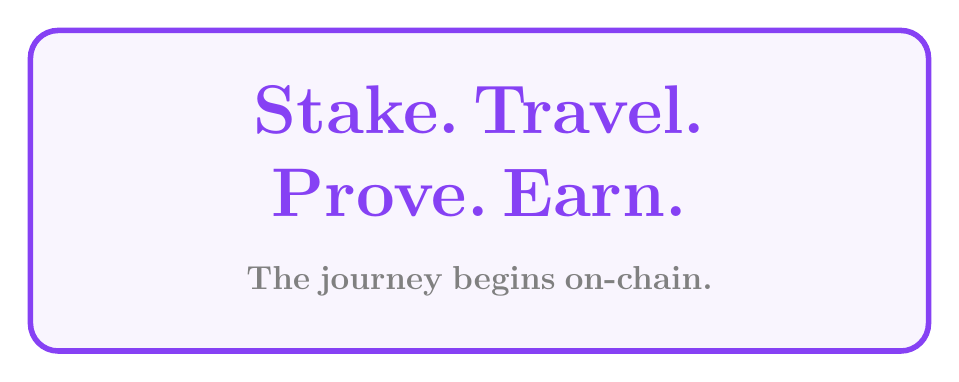
\begin{tikzpicture}
    \node[
        rectangle,
        rounded corners=10pt,
        draw=monadPurple,
        line width=2pt,
        fill=monadPurple!5,
        text width=10cm,
        align=center,
        inner sep=20pt
    ] {
        \Huge\bfseries\textcolor{monadPurple}{Stake. Travel. Prove. Earn.}\\[0.5cm]
        \large\textcolor{gray}{The journey begins on-chain.}
    };
\end{tikzpicture}
\end{center}

% ============================================
% REFERENCES
% ============================================
\newpage
\section*{References \& Resources}

\begin{itemize}
    \item \textbf{Monad Documentation:} \url{https://docs.monad.xyz}
    \item \textbf{Foundry Book:} \url{https://book.getfoundry.sh}
    \item \textbf{OpenZeppelin Contracts:} \url{https://docs.openzeppelin.com/contracts}
    \item \textbf{Wagmi Documentation:} \url{https://wagmi.sh}
    \item \textbf{Leaflet Maps:} \url{https://leafletjs.com}
    \item \textbf{Wanderify App:} \url{https://wandryfi.vercel.app}
    \item \textbf{Backend API:} \url{https://wandrify.onrender.com}
\end{itemize}

\vspace{1cm}

\begin{center}
\textit{Wanderify Protocol Whitepaper v1.0}\\
\textit{January 2026}\\
\vspace{0.5cm}
\textbf{License:} MIT
\end{center}

\end{document}
